\chapter{The First Chapter}
\label{chap:first}
\begin{document}

\chapter{Thew Exploratory Data Analysis}
\label{chap:chapter4}

\section{Introduction}

The use of social media technology tools in government can be effective to  achieve digital footprint to streamline the delivery of services and user engagement.  The research study initiates by exploratory analysis of Twitter data set generated by users for a period from 2016 to 2021, indirectly generating big data and through analytics capabilities to uncover hidden patterns from historical data to aid future decision making.   The outcomes of the chapter is mainly comprised of firstly descriptive aspects an analytic process to uncover twitter behavioural characteristics to address first RQ1. This is done by measuring engagement between government and public users on twitter, by exploring features and trends of behaviour over time.  Secondly to answer the RQ2, with further reviewing overall trending topics for the four year summarised to provide insights of past conversations and determined sentiments ratings as results from text mining of a tax government department in analytic outcomes.  Overall outcome of the chapter will guide necessary machine learning use (RQ3) for future solution based on hindsight from data insight in understanding engagement, behaviour characteristics for participation for effective use of Twitter by the government agency to make a difference.\\

\section{User: Government Agency}

With the government agency as Twitter user with an interaction with citizens with rigour from 2018 to 2021 has accumulated in 7 896 messages indicating a strategy of customer service agency, a transactional tactic based on a dedicated social media team that can offer individualised responses as shown by the analysis.

The exploration of social media data through analytics is an important step to understand engagement behaviour between users as contributors to the data.  This data has been acted upon for exploring data characteristics aspects and features such as likes, retweeted messages, replies messages while providing understanding at a glance engagement aspects up to the topics and overall sentiments.  Therefore, the framework that has guided the research methods for the study data analysis and experiment needed is the ground theory approach guided by the exploratory analysis results.  This approach has discovered that users tweets have little usage of hashtags, thus resulting in a hashtag recommendation system to optimize effective use of social media for tweets for the government department under a decade of using twitter.\\
By looking at the average impressions of the number of times a tweet has been seen by users on the social media platform," to track the reach and engagements of tweets to determine the impact of their content on Twitter.\\
The user activity in terms of time is at the highest early hours of the morning, from 05h00 until midday, while seems to stop at about 9pm.\\
The user data does not contain any retweets.  Hence any other duplicates were removed for an amount of 7 867 tweets originating from the government agency.\\
Overall, about 26 percent (2 059)of tweets have not been replied to, meaning the more than 70 percent of tweets have been replied to by the government agency in relation to its social media policy.  This implies a customer service Twitter Strategy for a government department with dedicated staff responding to tweets with assistance of knowledge experts inside the organisation.\\

\begin{itemize}
    \item User participation (Time and Months)
\end{itemize}

Average impressions per tweet by hour tweeted:
----------------------------------------------
12 - 13 : 0.0 = 487 tweets\\
11 - 12 : 0.0 = 675 tweets\\
 8 - 9  : 0.0 = 707 tweets\\
 7 - 8  : 0.0 = 826 tweets\\
 6 - 7  : 0.0 = 957 tweets\\
 5 - 6  : 0.0 = 1361 tweets\\
14 - 15 : 0.0 = 126 tweets\\
10 - 11 : 0.0 = 730 tweets\\
 4 - 5  : 0.0 = 681 tweets\\
13 - 14 : 0.0 = 252 tweets\\
 9 - 10 : 0.0 = 793 tweets\\
 3 - 4  : 0.0 = 111 tweets\\
15 - 16 : 0.0 = 53 tweets\\
16 - 17 : 0.0 = 23 tweets\\
18 - 19 : 0.0 = 4  tweets\\
20 - 21 : 0.0 = 3  tweets\\
 2 - 3  : 0.0 = 49 tweets\\
 1 - 2  : 0.0 = 20 tweets\\
17 - 18 : 0.0 = 18 tweets\\
19 - 20 : 0.0 = 1  tweets\\

Time trends show an urgency dedicated to customer service department strategy with engagement of more than 12 hours in a day.   The first year for the user (department) Twitter full implementation of social media strategy in 2016 as evidently shown in fig 1, since then  there has been a sturdy increase in its usage, in all the 4 yeas shown the most busiest months are mainly July, August, September and October.  These are months associated with individual filing of returns for the tax Season which starts in July.\\

\begin{figure}
      \centering
	    \begin{subfigure}{0.3\linewidth}
		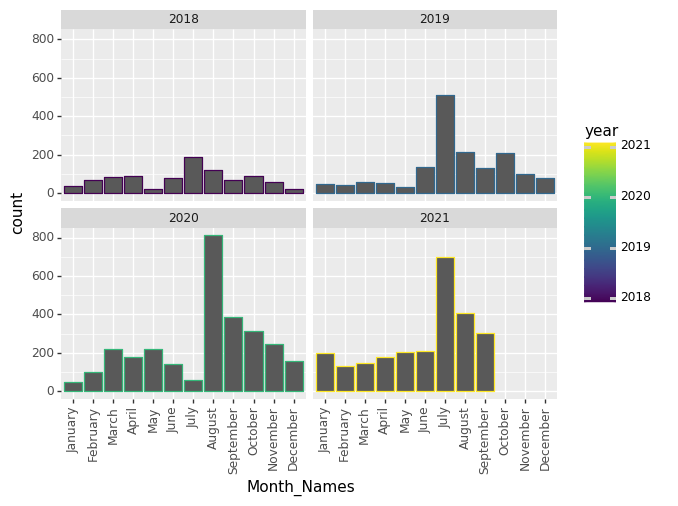
\includegraphics[width=\linewidth]{Users Month Names.png}
		\caption{Monthly engagements}
		\label{fig: Monthly Breakdown for engagement}
	   \end{subfigure}
	   \begin{subfigure}{0.3\linewidth}
		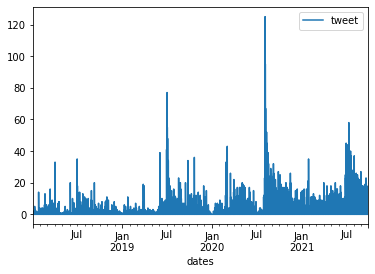
\includegraphics[width=\linewidth]{User 1 Minute Count.png}
		\caption{Time trends outputs}
		\label{fig:Breakdown of time trends by minute}
	    \end{subfigure}
	   \vfill
	 \caption{Time Comparison Monthly vs. Minutes in user engagement.}
\end{figure}

\begin{itemize}
    \item Hashtag Analysis
\end{itemize}

Another aspect to consider is hashtag use, in total for the 7 867 unique records of tweets, only 729 tweets have some representation of hashtags, meaning that 91 percent of tweets do not have any hashtags.  As a result of peaks in Twitter during the tax season for submission of returns by individuals, despite less than 15 percent of tweets use hashtags. The most popular used hashtags are in relation to the context of the filing season, YourTaxMatters(219), SARSTaxTips19(48), TaxSeason2018 (26), SARSRevenueAnnouncement(24), BRICS10Customs(22).\\

\begin{figure}
    \centering
    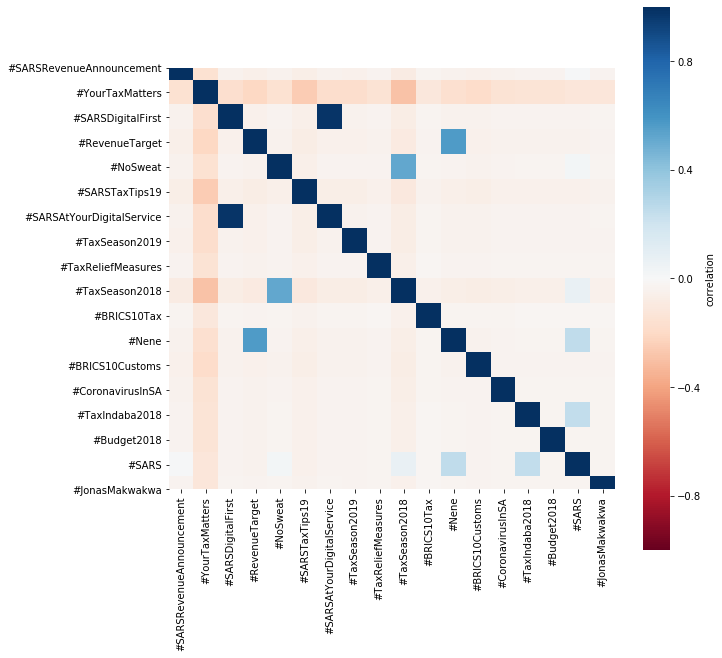
\includegraphics[width=0.1\linewidth]{User Hashtag Correlation.png}
    \caption{Hashtag correlation output}
    \label{fig:Hashtag correlation for government user}
\end{figure}

The correlation matrix shows the following relationship between the most used hashtags
\begin{itemize}
    \item SARSTaxTips19 has a strong positive relationship with YourTaxMatters.  
    \item TaxSeason2018 has a negative relationship with YourTaxMatters.  
    \item TaxSeason2018 has a strong positive relationship with Nosweat
    \item  Nene has a positive relationship with RevenueTarget
    \item  Nene has a positive relationship with SARS 
\end{itemize}

This could mean sending of tax tips in 2019 tax year were helpful for the tax season activities.  The 2018 tax season was not so instrumental.  However, at the same time for the 2018 with a strong support of no sweat campaigns.  Nene had a favourable revenue announcement for tax collection and with SARS in general.

\begin{figure}
      \centering
	    \begin{subfigure}{0.3\linewidth}
		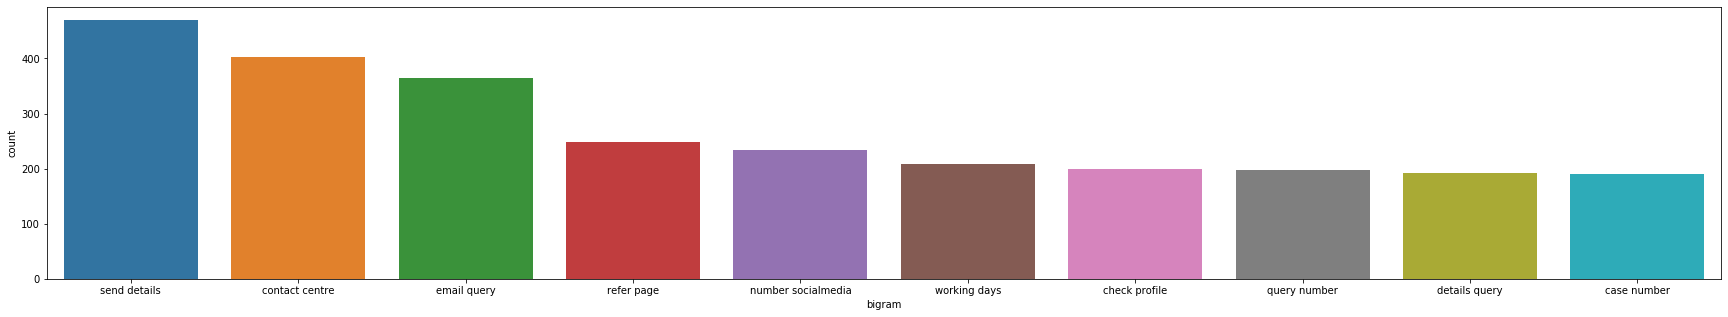
\includegraphics[width=\linewidth]{Bigrams User Data.png}
		\caption{Bi-Grams outputs for government User}
		\label{fig: Associated Bi-Grams Outputs}
	   \end{subfigure}
	   \begin{subfigure}{0.3\linewidth}
		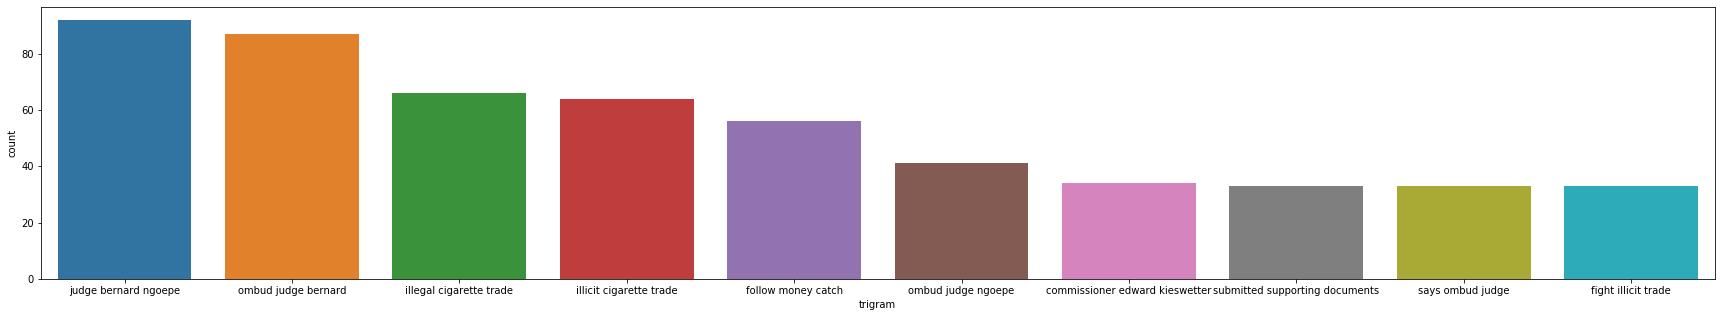
\includegraphics[width=\linewidth]{Tri-gram User Data.png}
		\caption{Tri-Grams outputs for government User}
		\label{fig:Associated Tri-Gram Outputs}
	    \end{subfigure}
	   \vfill
	 \caption{Comparing Bi-Gram vs. Tr-Grams in Phrase Modelling for government user data.}
\end{figure}

Shown by fig 3, with most tweets not containing hashtags the phrase modelling technique was used to assist highlight context of messages by making use of the bi-gram and tri-gram outputs. Mostly, the 2 words which appear together in the top 10 bi-grams coincides with the queries users must have imposed that are service related to the PIT filing season, which indicates that the strategy of customer service oriented government department.  The tri-grams indicate citizens engaging with the department mandate, governance and operations concerns.

Overall, based on the table below few interesting characteristics based on the 7 867 messages.
\begin{itemize}
    \item For every tweet comes with one reply on average. This implies a strategy for social media in a government department that is dedicated to customer service, and responding individually to messages guided by policies.  The outlier shown by a maximum figure of 137 replies relates to a 2021 announcement on,  "We are pleased to announce that a SARS browser solution is now available following issues experienced with the discontinuation of Adobe Flash Player. Thread"
    \item On average every tweet comes retweeted twice.  The outlier of 986 replies is for an announcement on WE ARE HIRING! Some of the capable and highly skilled individuals we need to join us on this exciting journey are: • Chief Data Scientist • Chief Technology &amp; Innovation Officer • Chief Financial Officer • Chief Procurement Officer • Chief Litigation Officer.
    \item On average every tweet comes with 2 likes.
    \item on average tweets are emerging mainly from the 2019 year.
    \item As seen in Fig 5.1 July and August are the most months.
\end{itemize}

\section{User: Citizens}\\

The 7 867 government agency tweets have resulted in 
66 976 tweets data conversation sets with interesting characteristics to monitor engagements for metrics to be examined such as retweets, replies, hashtags, direct messages and overall impact of tweets. 

\begin{itemize}
    \item Time Trends
\end{itemize}

The data description for the 10 year range produced about 66919 entries, with 34 features,  of which 98percent of the data  is for the last 4 years that is 2018 to 2021.  The majority of tweets were observed in the 2021 year, followed by 2020.In 2018 the government agency seem to have strengthened strategy especially on twitter for a business value that is based on relationship building and offering instant support to citizens.\\

\begin{figure}
      \centering
	    \begin{subfigure}{0.1\linewidth}
		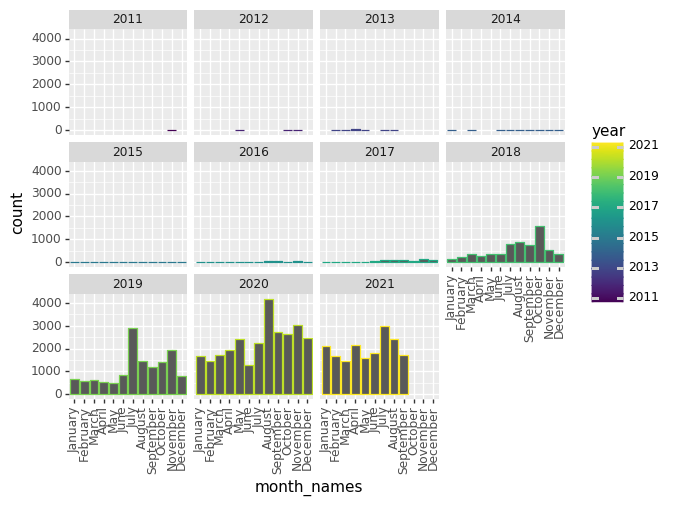
\includegraphics[width=\linewidth]{Overall 10 years of data.png}
		\caption{Overall 10 years}
		\label{fig: 10 year data distribution}
	   \end{subfigure}
	   \begin{subfigure}{0.1\linewidth}
		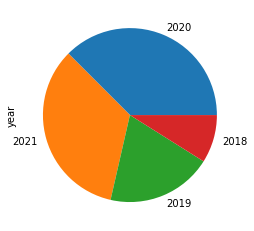
\includegraphics[width=\linewidth]{Annual trends Second Data.png}
		\caption{Four years}
		\label{fig:Four years}
	    \end{subfigure}
	   \vfill
	 \caption{}
\end{figure}

As a result of customer service Twitter strategy the stats below indicate that tweet movement starts early hours in the morning from 5am and gradually slows down early evening at about 7pm, overall users are engaged through out the 24 hour period as shown below.  

Average impressions per tweet by hour tweeted:
----------------------------------------------
20 - 21 : 0.0 =>  525 tweets\\
19 - 20 : 0.0 =>  955 tweets\\
17 - 18 : 0.0 => 2483 tweets\\
15 - 16 : 0.0 => 2965 tweets\\
14 - 15 : 0.0 => 2885 tweets\\
13 - 14 : 0.0 => 3214 tweets\\
12 - 13 : 0.0 => 3766 tweets\\
11 - 12 : 0.0 => 4204 tweets\\
10 - 11 : 0.0 => 4373 tweets\\
 9 - 10 : 0.0 => 4717 tweets\\
 8 -  9 : 0.0 => 4885 tweets\\
 7 -  8 : 0.0 => 5298 tweets\\
 6 -  7 : 0.0 => 5393 tweets\\
 5 -  6 : 0.0 => 5708 tweets\\
 4 -  5 : 0.0 => 4248 tweets\\
 2 -  3 : 0.0 => 1310 tweets\\
21 - 22 : 0.0 =>  291 tweets\\
18 - 19 : 0.0 => 1759 tweets\\
16 - 17 : 0.0 => 2893 tweets\\
 3 -  4 : 0.0 => 2536 tweets\\
 1 -  2 : 0.0 =>  688 tweets\\
 0 -  1 : 0.0 =>  234 tweets\\
23 - 24 : 0.0 =>  211 tweets\\
22 - 23 : 0.0 =>  224 tweets\\

While above it was discussed that on average every tweet posted results in one reply and three likes, some of the tweets may not be responded due to not relating to the specific topic that the customer service oriented government strategy cannot respond to.  However, the point that limited use of hashtags in tweets can result in majority of messages not aligned to a specific topic is valid, with better use of hashtags can effectively connect social media content to a specific topic or event.

\begin{itemize}
    \item Hashtag Analysis
\end{itemize}

More than 80 percentage of the tweets do not have hashtags.  Of those with hashtags used less than 20 percent comes with a possibility of messages not relating to the topic. Overall it would be interesting if the topic modelling results for topics fall within the parameters of the  government agency.

\begin{figure}
    \centering
    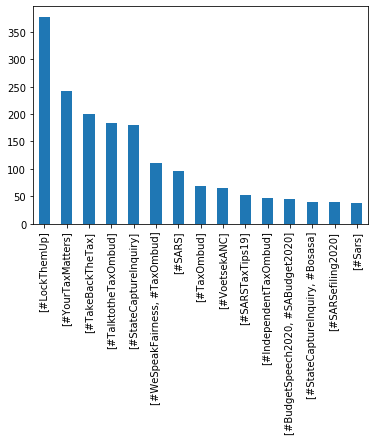
\includegraphics[width=0.1\linewidth]{Hashtags Used Second Data .png}
    \caption{Enter Caption}
    \label{fig:enter-label}
\end{figure}

As seen in Figure 8 below the majority of the communication came though the filing season or campaigns for submissions of returns by individuals taxpayers which occurs mainly between July to September, slowing down in October. This period has the most significant usage of hashtags, such as YourTaxMatters, TaxSeason and with other tax season non-related hashtags such as lockthemup and Statecaptureenquiry.  The tax season hashtags dominating in this period have been following the same trend but higher especially in 2021, which is the year with most tweets for the four main years under study. 

\cite{alsini2021hashtag} It can be beneficial to have correct use of hashtags to contextualize conversations to focus on better engagement(s).  This can lead to greater and quick engagement in users boosting the brand’s social media engagement through likes, shares, comments, and a potential of new followers. Also to bring other topics that may not be important outside the tax season, while eliminating noise and information overload.

\begin{itemize}
    \item Username Analysis
\end{itemize}

It is interesting to note that the dominating usernames other than the "sarstax" are from public figures including tax practitioners - username distribution over the 4-year period shows mainly engagements with civil societies, journalists, tax practitioners, government officials in the public space due to various political reasons.  

\begin{figure}
    \centering
    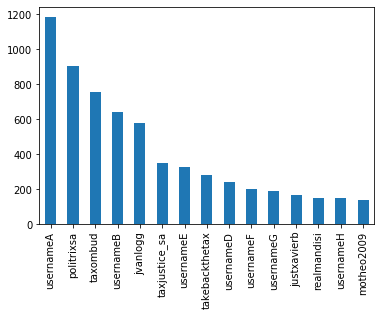
\includegraphics[width=0.1\linewidth]{usenames for second data.png}
    \caption{Enter Caption}
    \label{fig:enter-label}
\end{figure}

\begin{itemize}
    \item Topics 
\end{itemize}

\begin{itemize}
    \item Phrase modelling outputs
\end{itemize}


Looking at the phrase modelling outputs, the tri-grams visualisation output of the top 10 for 3 words which frequently appear together indicates a summary of interesting topics relating to strategy matters.

\begin{figure}
      \centering
	    \begin{subfigure}{0.1\linewidth}
		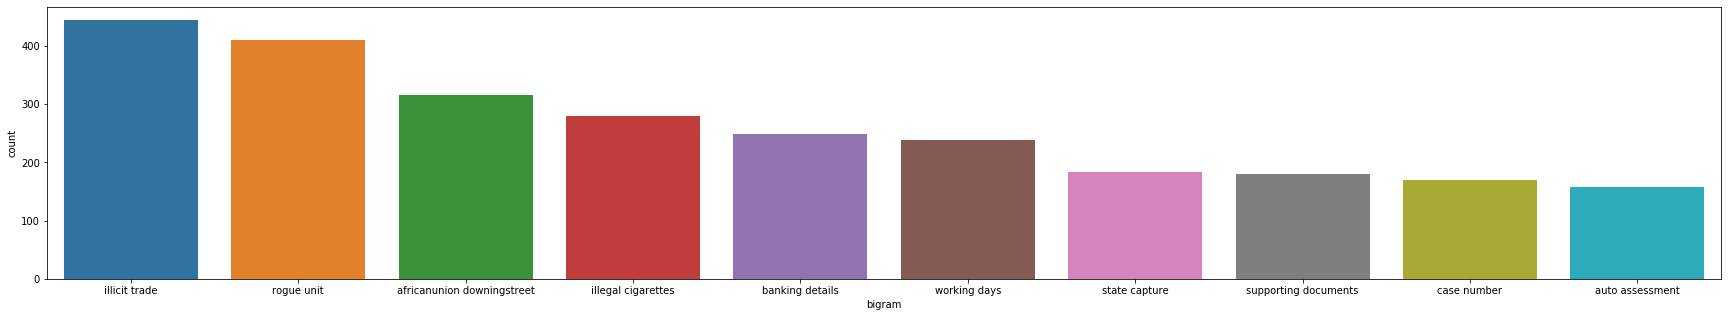
\includegraphics[width=\linewidth]{Bi-grams for second second user data.png}
		\caption{Bi-Grams outputs}
		\label{fig: Associated Bi-Grams Outputs}
	   \end{subfigure}
	   \begin{subfigure}{0.3\linewidth}
		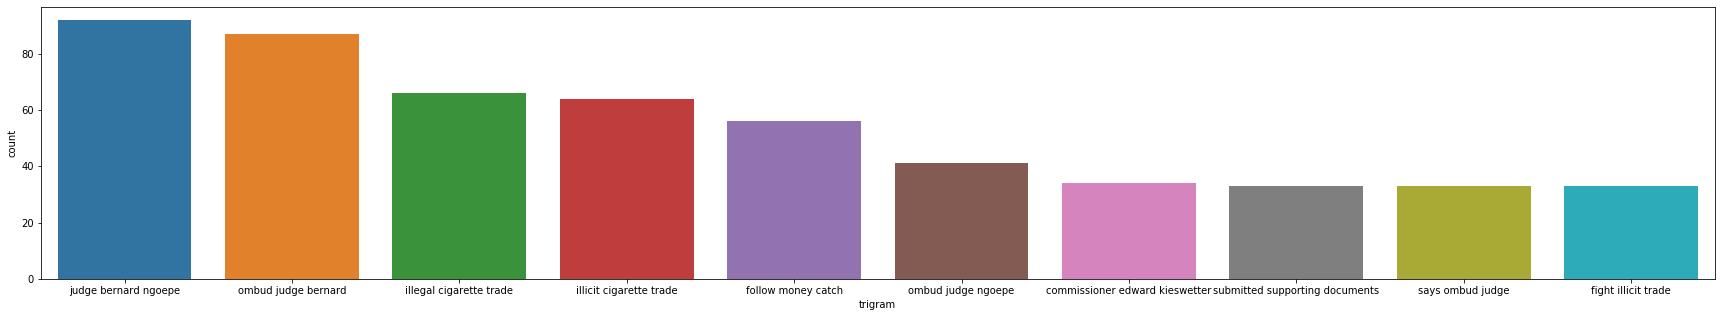
\includegraphics[width=\linewidth]{Tri-gram second second user data.png}
		\caption{Tri-Grams outputs}
		\label{fig:Associated Tri-Gram Outputs}
	    \end{subfigure}
	   \vfill
	 \caption{Comparing Bi-Gram vs. Tr-Grams in Phrase Modelling.}
\end{figure}

Whereas, the bi-grams visualisation for the 2 words which frequently appear together are tax service related on matters taxpayers needed clarity on.

\begin{itemize}
    \item Emerging topics from text analysis
\end{itemize}

The text analysis technique that has been leveraged on to deduce a list of possible topics resulting from overall corpus is the LDA Topic Modelling Technique.  In comparison to other unsupervised topic models algorithms such as the Latent Semantic Indexing (LSI), Hierarchical Dirichlet Process (HDP).  The LDA is more reliable to produce coherent and quality topics when evaluating results with other models as it shows to have better coherence metric values, as shown below.\\

\begin{figure}
      \centering
	    \begin{subfigure}{0.1\linewidth}
		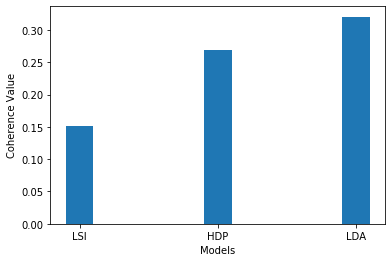
\includegraphics[width=\linewidth]{Evaluate coherence values.png}
		\caption{Coherence values performance }
		\label{fig: Coherence Values}
	   \end{subfigure}
	   \begin{subfigure}{0.1\linewidth}
		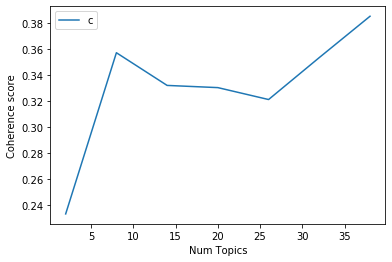
\includegraphics[width=\linewidth]{Number of Topics for the overall data.png}
		\caption{Visual representation of Number of Topics}
		\label{fig:Number of Topics selection}
	    \end{subfigure}
	   \vfill
	 \caption{Comparing topic models coherence values vs  number of topics}
\end{figure}

In order to get the main themes for created topics resulting from the LDA algorithms the process start with the best choice parameters for a finer model by running the CV grid search method to find the best parameters for the LDA.  To initialize  involves feature extraction from the document term matrix of a TF-IDF vector to carry out the topic modelling. The matrix comes with a sparsicity of 0,48 percent following the data processing and removal of stop words, last consideration is the maximum features of 1000.\\
As shown above in fig 9 clearly that the parameter for number of topics =with a value of 10 has a better score for the coherence score of 0.36.\\

Overall results therefore, the base LDA model has the final hyperparameters based on CV Grid search method as follows, the number of topics=10, the learning method for the algorithm updating the assignment of topics to the documents=online, together with the maximum number of iterations to be carried out =10 and the random state = 100.\\
The results are 10 distinct topics despite some topics could share common keywords, it may help to checking for proportion of assigned topics by the model.  In checking the results we can check the proportion of topics that have been assigned to the first document using the lines of code given below.

The table below shows that Topic 10 has the highest proportion

Proportions of topics from the document:\\
\begin{itemize}
    \item Topic  0 :  5.0000000003264145 %\\
\end{itemize}
\begin{itemize}
    \item Topic  1 :  5.000530695799997 %\\
\end{itemize}
\begin{itemize}
    \item Topic  2 :  5.001280907842061 %\\
\end{itemize}
\begin{itemize}
    \item Topic  3 :  5.000000000379809 %\\
\end{itemize}
\begin{itemize}
    \item Topic  4 :  5.0002008679359955 %\\
\end{itemize}
\begin{itemize}
    \item Topic  5 :  5.000000000399167 %\\
\end{itemize}
\begin{itemize}
    \item Topic  6 :  5.000000000336659 %\\
\end{itemize}
\begin{itemize}
    \item Topic  7 :  5.000000000286975 %\\
\end{itemize}
\begin{itemize}
    \item Topic  8 :  5.00028074430452 %\\
\end{itemize}
\begin{itemize}
    \item Topic  9 :  54.9977067823884 %\\
\end{itemize}

For the following 10 topics resulting in the topic modelling LDA technique the results are listed below:

\begin{itemize}
    \item Topic 0: trade report illicit true follow criminals state zuma million reason
\end{itemize}
\begin{itemize}
    \item Topic 1: return working days long audit refund guys returns months year
\end{itemize}
\begin{itemize}
    \item Topic 2: number efiling waiting branch assist submit received today documents response
\end{itemize}
\begin{itemize}
    \item Topic 3: good hope refunds look company file things issue pravin police
\end{itemize}
\begin{itemize}
    \item Topic 4: thank thanks ombud customs exactly believe email address sent compliance
\end{itemize}
\begin{itemize}
    \item Topic 5: unit right commissioner sure start great maybe rogue point minister
\end{itemize}
\begin{itemize}
    \item Topic 6: people problem country like really public question wrong getting white
\end{itemize}
\begin{itemize}
    \item Topic 7: cigarettes paid going paying free taxes read open crime president
\end{itemize}
\begin{itemize}
    \item Topic 8: government illegal corruption business black check court dont evidence years
\end{itemize}
\begin{itemize}
    \item Topic 9: come money stop want details know time need help tell
\end{itemize}

Therefore the topic 10 listed topics from the corpus are listed below as:

When using human judgements to determine the topics are as follows:
\begin{itemize}
    \item Topic 1:  Fight illegal trade activity 
\end{itemize}
\begin{itemize}
    \item Topic 2: long turnaround times post returns submission
\end{itemize}
\begin{itemize}
    \item Topic 3: Minister appointment of commissioner
\end{itemize}
\begin{itemize}
    \item Topic 4:  Appreciatiing tax ombud results
\end{itemize}
\begin{itemize}
    \item Topic 5: Hope for tax refunds appropriateness
\end{itemize}
\begin{itemize}
    \item Topic 6: Minister address rogue unit 
\end{itemize}
\begin{itemize}
    \item Topic 7: Urgent llicit cigarette trade tax crime 
\end{itemize}
\begin{itemize}
    \item Topic 8: Government corruption loosing battle in providing evidence
\end{itemize}
\begin{itemize}
    \item Topic 9:  assistance required case number to query details 
\end{itemize}

Overall the topics discovered through the topic modelling LDA technique realte to the activities for the four years covered. 

\begin{itemize}
    \item Sentiment outputs from text analysis
\end{itemize}

Having explored possible topics from the 4 year engagement discussions, the next is sentiment analysis for overall breakdown engagement of reactions and inputs from users online interaction that can add up emotions from messages with the government department experience over the years covered in the study.  This is to add some quantitative metrics through sentiment analysis in the data exploration analysis.

As messaged add up based on social media use and analysing users comments overtime using a VADER function in python software for a Natural Language Processing (NLP) technique.  
The VADER (Valence Aware Dictionary and sEntiment Reasoner) is a lexicon and rule-based sentiment analysis library of the SentimentIntensityAnalyzer class in Python which returns 4 values, pos, neu, neg and compound.  The compound score is normalised rating of the pos, neu and neg ratings for a single metric value to determine a sentiment. 

The algorithm returns sentiment rating for each tweet for positive, negative and neutral and a compound value to provide a general sentiment of the string.  
While fig 5.14 shows distribution of the normalised compound scores that provides basis for the overall sentiment metric, the actual sentiment scores shows higher neutral sentiments, followed by positive with narrow margin, however the negative sentiment is lowest as shown by Fig 5.15.  At the same time the trend seem to be the same actoss all months of the calendar year depicted in Fig 5.16.\\

\begin{figure}
      \centering
	    \begin{subfigure}{0.1\linewidth}
		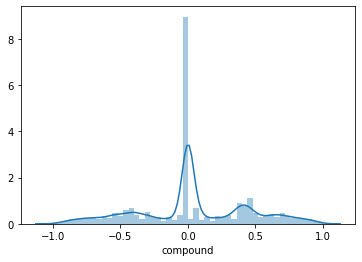
\includegraphics[width=\linewidth]{Sentiment Compound 2.png}
		\caption{Compound results}
		\label{fig:subfig1}
	   \end{subfigure}
	   \begin{subfigure}{0.1\linewidth}
		\includegraphics[width=\linewidth]{Overall Sentiment 2.png}
		\caption{Monthly Sentiments Rating}
		\label{fig:subfig2}
	    \end{subfigure}
	   \vfill
	   \begin{subfigure}{0.1\linewidth}
	   \includegraphics[width=\linewidth]{Overall Sentiments.png}
	   \caption{Overall Sentiment Rating}
	   \label{fig:subfig3}
	   \end{subfigure}
	 \caption{Comparing blue car vs. red car.}
\end{figure}

In all each tweet message has been classified and scored into a sentiment metric of either positive, negative or neutral to get an overview of citizens emotions on their engagements.  It is also possible to observe the sentiments related with the hashtags for the few tweets that have hashtags as shown in Figure and Figure for positive and negative sentiments:\\

\begin{figure}
      \centering
	    \begin{subfigure}{0.1\linewidth}
		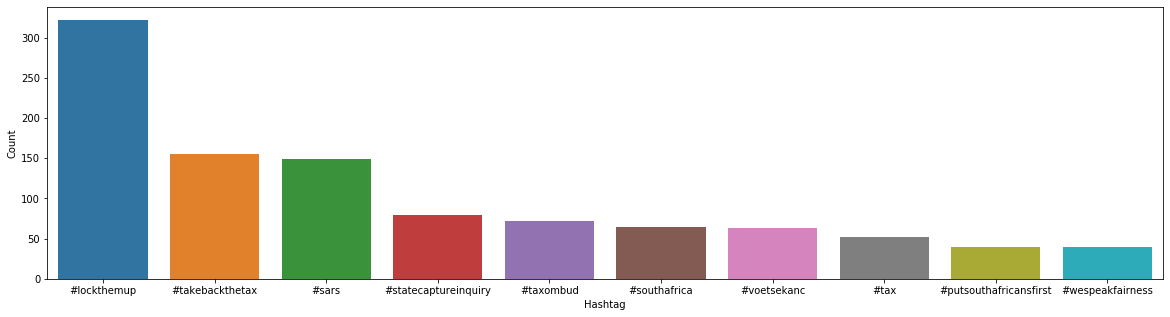
\includegraphics[width=\linewidth]{Sentiments Hashtag Negative.png}
		\caption{Hashtags associated with negative sentiments}
		\label{fig:subfig1}
	   \end{subfigure}
	   \begin{subfigure}{0.1\linewidth}
		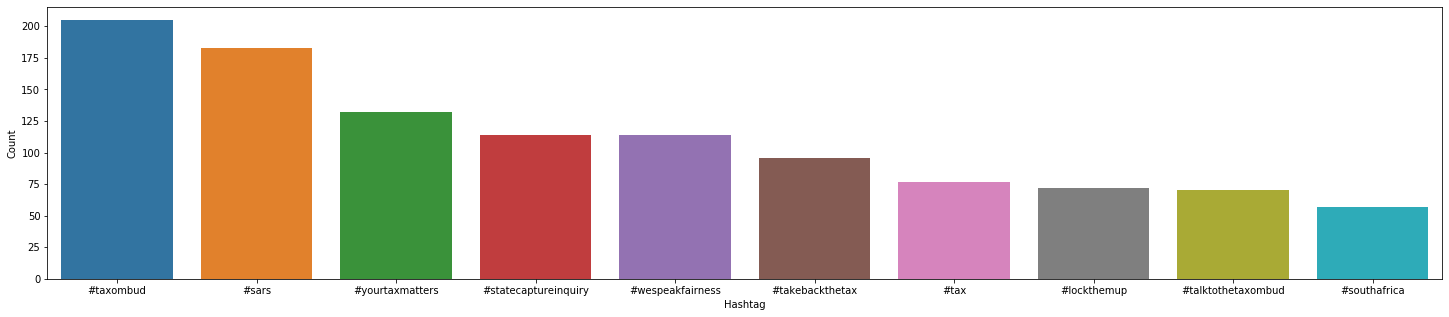
\includegraphics[width=\linewidth]{Hashtag Sentiments Positive.png}
		\caption{Hashtags associated with positive sentiments}
		\label{fig:subfig2}
	    \end{subfigure}
	   \vfill
	 \caption{Comparing blue Negative vs. Positive Sentiment Hashtags.}
\end{figure}

In applying human judgement the possibility of hashtags associated with the sentiments are validated to align\\ 

\subsubsection{Conclusion}

The results of the chapter aim to answer RQ1 abd RQ2 by covering qualitative findings through an exploratory data analysis that has produced results providing insights, understanding including characteristics and behavioural engagements measured between the users, a government and  citizens.\\  Through the ground theory approach for the analysis has revealed results amongst others that users tweets have little usage of hashtags, thus resulting in a hashtag recommendation system to optimise effective use of social media for tweets for the government department under a decade of using twitter.  This chapter is important to give context to the proposed hashtag recommendation solution as a need from the results of user engagements from historical factors.  

\end{document}